\documentclass[12pt]{article}
\usepackage{fontspec}
\usepackage{amsfonts}
\usepackage{amsmath}
\usepackage{yfonts}
\usepackage{polyglossia}
\usepackage{color}
\usepackage{hyperref}
\usepackage{ifthen}
\usepackage{pdfcomment}
\defaultfontfeatures{Ligatures=TeX}

\title{E\\Słownik Lindego t. I s. 756}
\author{Jarosław Kopiński (red.)}
\date{\today}

\newcommand{\doh}[1]{⸗}

\newcommand{\biblio}[4]{#1\footnote{#2\ifthenelse{\equal{#2}{}}{}{, }#3} #4}

\newcommand{\ti}{\textit}
\newcommand{\ind}{\indent}
\newcommand{\nin}{\noindent}
\newcommand{\nind}{\newline\indent}
\newcommand{\nl}{\newline}

\catcode`\&=12

\setmainfont{Linux Libertine O}
\setmonofont{DejaVu Sans Mono}

\begin{document}

\maketitle


\url{http://teksty.klf.uw.edu.pl/25/3/LindeIIGP%2B1i.djvu?djvuopts=&page=756&zoom=width&showposition=0.5,0.44}

\bigskip
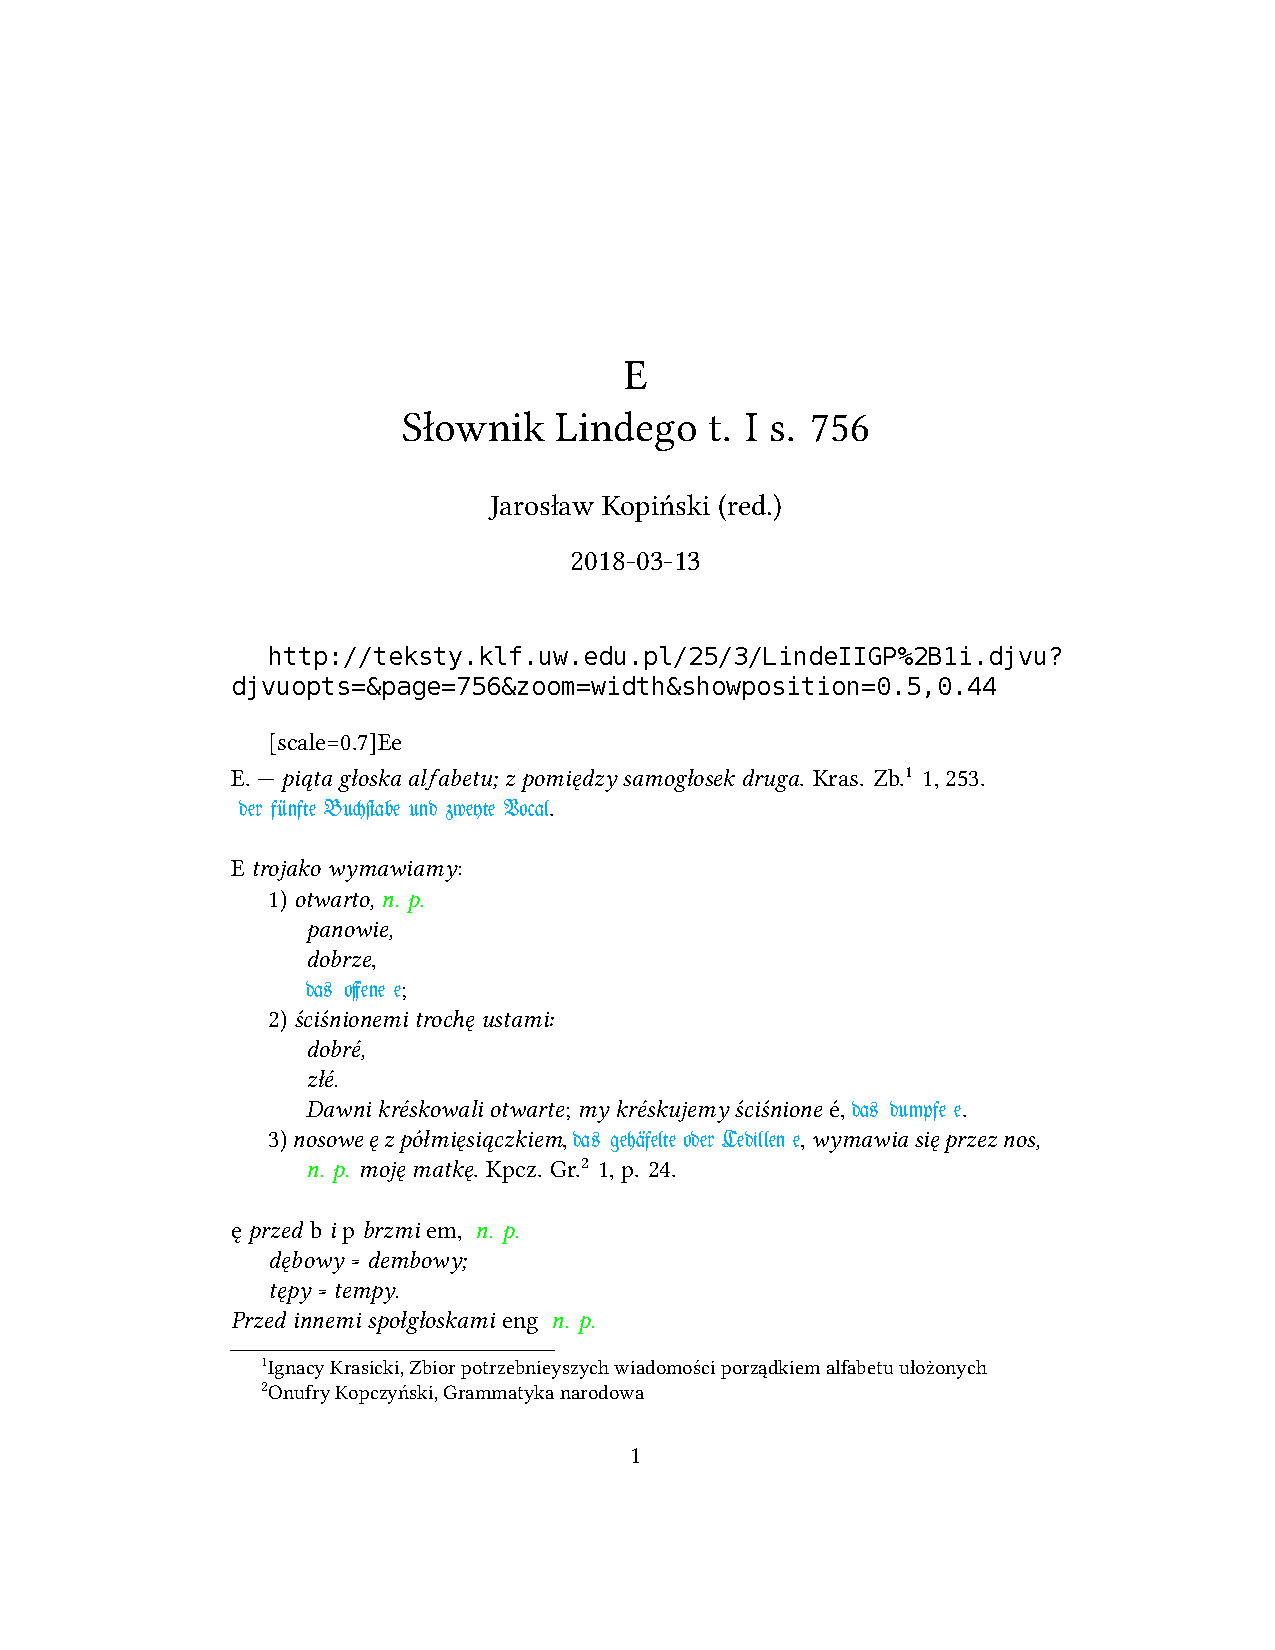
\includegraphics[scale=0.7]{Ee}

\smallskip


\nin
E. --- \ti{piąta głoska alƒabetu; z pomiędzy samogłosek druga}.
\biblio{Kras. Zb.}{Ignacy Krasicki}{Zbior potrzebnieyszych wiadomości porządkiem alfabetu ułożonych}{1, 253}.
\nl
\pdftooltip{\textcolor{cyan}{\textfrak{ der f"unfte Buchstabe und zweyte Vocal}}}{der funfte Buchstabe und zweyte Vocal}.
\nl \nl
\nin
E \ti{trojako wymawiamy}:
\nind
1) \ti{otwarto, \pdftooltip{\textcolor{green}{n. p.}}{na przykład}
\nind \ind
panowie,
\nind \ind
dobrze},
\nind \ind %W poniższej linii znajduje się trudny do zidentyfikowania znak (przed e)
\pdftooltip{\textcolor{cyan}{\textfrak{das: offene e}}}{das offene e};
\nind
2) \ti{ściśnionemi trochę ustami:
\nind \ind
dobré,
\nind \ind
złé.
\nind \ind
Dawni kréskowali otwarte}; \ti{my kréskujemy ściśnione} é, \pdftooltip{\textcolor{cyan}{\textfrak{das: dumpfe e}}}{das dumpfe e}.
\nind
3) \ti{nosowe ę z półmięsiączkiem}, \pdftooltip{\textcolor{cyan}{\textfrak{das: geh"afelte oder Cedillen e}}}{das gehafelte oder Cedillen e}, \ti{wymawia się przez nos, 
\ind \ind
\pdftooltip{\textcolor{green}{n. p.}}{na przykład} moję matkę}. \biblio{Kpcz. Gr.}{Onufry Kopczyński}{Grammatyka narodowa}{1, p. 24}.
\nl
\nl
ę \ti{przed} b \ti{i} p \ti{brzmi} em, \ti{ \pdftooltip{\textcolor{green}{n. p.}}{na przykład}}
\nind
\ti{dębowy} \doh{} \ti{dembowy;
\nind
tępy} \doh{} \ti{tempy.}
\nl
\ti{Przed innemi społgłoskami} eng \ti{ \pdftooltip{\textcolor{green}{n. p.}}{na przykład}}
\nind
\ti{męka} \doh{} \ti{mengka;
\nind
ręka} \doh{} \ti{rengka}; 
\newline
\ti{na końcu słów ledwie co slychać różnicy} ę \ti{od é \pdftooltip{\textcolor{green}{n. p.}}{na przykład}
\nind
idę,
\nind
gotuję,
\nind
matkę.} --- 
\newline
Januszowski \ti{prócz tych, czwarte jeszcze najduje, \pdftooltip{\textcolor{green}{n. p.}}{na przykład} w słowach paniéj ochotnéj; i temu naznacza kréskę od prawéj do lewéj; otwartemu zaś od lewéj do prawéj, w czém się i od} \pdftooltip{J. Kchan.}{Jana Kochanowskiego} \ti{i od} \pdftooltip{Łuk. Gornickiego}{Łukasza Gornickiego} \ti{odstrzela}. \biblio{Nowy Char.}{Jan Januszowski}{Nowy Charakter Polski} {(\pdftooltip{\textcolor{blue}{\ti{cf.}}}{confer} Not. \pdftooltip{\textcolor{blue}{\ti{ad lit.}}}{ad litem} a, à, ą).\pdftooltip{\textcolor{blue}{\ti{NB}}}{Nota Bene}.}
\newline
\ti{Niemasz żadnego słowa prawdziwie Polskiego, ktoreby się od} e \ti{zaczynało;} 
\newline
\indent
Elbląg, \ti{osada Lubecka, imię nadane sobie miał przez Niemców;}
\newline
\indent
ejnał, hejnał, \ti{Węgierskie jest słowo.}
\newline
\ti{Pochodzi to ztąd, że czém u Greków \textcolor{blue}{spiritus asper}, tém u nas jest} j, ch, h.
\end{document}
%%% Local Variables: 
%%% coding: utf-8-unix
%%% mode: latex
%%% TeX-master: t
%%% TeX-PDF-mode: t
%%% TeX-engine: xetex
%%% End: 
